 %%%%%%%%%%%%%%%%%%%%%%%%%%%%%%%%%%%%%%%%%%%%%%%%%%%%%%%%%%%%
%% This Beamer template was created by Cameron Bracken.
%% Anyone can freely use or modify it for any purpose
%% without attribution.
%%
%% Last Modified: January 9, 2009
%%
\documentclass[xcolor=x11names,compress,t]{beamer}
\usepackage{algorithm,algorithmic, color, tikz}
%% General document %%%%%%%%%%%%%%%%%%%%%%%%%%%%%%%%%
%%\usepackage{tikz}

\usepackage{array}

\usepackage{amssymb}% http://ctan.org/pkg/amssymb
\usepackage{graphicx}
% \usepackage[demo]{graphicx}
\usepackage{caption}
\usepackage{subcaption}
\usetikzlibrary{calc}
\usepackage[T1]{fontenc}
\usepackage[utf8]{inputenc}
\usepackage{textcomp}
\usepackage{eurosym}




%% Beamer Layout %%%%%%%%%%%%%%%%%%%%%%%%%%%%%%%%%%

\setbeamertemplate{navigation symbols}{}
%\setbeamertemplate{bibliography item}[text]
\setbeamercolor{block title}{bg=blue!40}
\setbeamercolor{block body}{bg=blue!20}

\useoutertheme[subsection=false,shadow]{miniframes}
\useinnertheme{default}
\usefonttheme{serif}
\usepackage{palatino}
\setbeamerfont{title like}{shape=\scshape}
\setbeamerfont{frametitle}{shape=\scshape}
\setbeamercolor*{lower separation line head}{bg=DeepSkyBlue4}
\setbeamercolor*{normal text}{fg=black,bg=white}
\setbeamercolor*{alerted text}{fg=red}
\setbeamercolor*{example text}{fg=black}
\setbeamercolor*{structure}{fg=black}
\setbeamercolor*{palette tertiary}{fg=black,bg=black!10}
\setbeamercolor*{palette quaternary}{fg=black,bg=black!10}

\renewcommand{\epsilon}{\varepsilon}
%%%%%%%%%%%%%%%%%%%%%%%%%%%%%%%%%%%%%%%%%%%%%%%%%%

\begin{document}

\begin{frame}
  \title{Chains and Antichains in the Bipartite Cambrian and Tamari Lattices}
  %\author{Eli Garcia, Rose Silver, Ben Drucker, Aubrey Rumbolt}
  \date{}
%  \institute{UCONN}

\vspace{-2 cm}

  \maketitle
  
  \vspace{-3 cm}
  
  \centering
  \begin{tabular}{c c c c}
  
    \includegraphics[width=.2\linewidth]{Ben.jpeg} &     \includegraphics[width=.2\linewidth]{Eli.jpeg}  & \includegraphics[width=.2\linewidth]{Aubrey.jpeg}  &
    \includegraphics[width=.2\linewidth]{Rose.jpeg} \\
    
    Ben Drucker & Eli Garcia & Aubrey Rumbolt & \textbf{Rose Silver} \\
    \end{tabular}
    
    \centering
    
    \vspace{1 cm}
    
    
    UCONN REU
\end{frame}
    



% \begin{frame}{Introduction to Partially Ordered Sets}
%     \begin{figure}
%     \centering
%         \begin{subfigure}{.5\textwidth}
%         \centering
%         \includegraphics[width=0.6\linewidth]{USDnotesNew.png}
%         \end{subfigure}%
%         \begin{subfigure}{.5\textwidth}
%         \centering
%         \includegraphics[width=0.6\linewidth]{Euro_banknotes,_Europa_series.png}
%         \end{subfigure}

%     \label{fig:test}
%     \end{figure}
    
%     \begin{itemize}
%         \item \textbf{Comparable:} $\$5 \leq \$10 \leq \$20$
%         \item \textbf{Comparable:} $5$\euro $\leq 10$\euro  $\leq 20$\euro
%         %\item \textbf{Incomparable:} $\$5$ vs 5\euro
%     \end{itemize}
% \end{frame}

%%What is a poset?
\begin{frame}{Posets}
    \begin{figure}[htp]
        \centering
        \includegraphics[scale = 0.14]{poset2.png}
    \end{figure}
    
    \textbf{Partially Ordered Set (Poset):} A set equipped with a relation $\leq$
\end{frame}

\begin{frame}{Comparing Elements in the Poset}
    \Huge
    \centering
    \vspace{1cm}
    $\{x,y\} \leq \{x,y,z\}$ \\
    \vspace{1cm}
    $\{x,y\} \nleq \{y,z\}$ 
\end{frame}

\begin{frame}{Posets}
    \begin{figure}[htp]
        \centering
        \includegraphics[scale = 0.14]{poset2.png}
    \end{figure}
    
    \textbf{Partially Ordered Set (Poset):} A set equipped with a relation $\leq$ \pause for which the following hold:
    
    \begin{enumerate}
        \item \emph{Reflexivity}: $a\leq a$
        
        \item \emph{Transitivity}: if $a\leq b$ and $b\leq c,$ then $a\leq c$
        
        \item \emph{Antisymmetry}: if $a\leq b$ and $b\leq a,$ then $a=b$
        
    \end{enumerate}
\end{frame}

\begin{frame}{Today's Talk}
    \begin{figure}
    \centering
        \begin{subfigure}{.5\textwidth}
        \centering
        \includegraphics[width=0.6\linewidth]{ExCambrianLattice.png}
        \end{subfigure}%
        \begin{subfigure}{.5\textwidth}
        \centering
        \includegraphics[width=0.6\linewidth]{Capture1.PNG}
        \end{subfigure}
    %\caption{Two different currencies}
    \label{fig:test}
    \end{figure}
    \begin{itemize}
        \item Describe the \underline{Bipartite Cambrian Lattice} \& \underline{Tamari Lattice}
        \item Prove interesting properties of these two posets
    \end{itemize}
    \vspace{1cm}
    \textcolor{blue}{Note: A lattice is a type of poset}
\end{frame}

\begin{frame}

\vspace{1 cm}

    \begin{center}
        \Huge
        \textbf{Part 1}\\
        The Bipartite Cambrian Lattice
        
        \vspace{3cm}
        \normalsize
        \textcolor{blue}{\textbf{[Reading; 2012]}}
    \end{center}

\end{frame}

\begin{frame}{Bipartite polygon ($n=6$)}
    \begin{figure}
        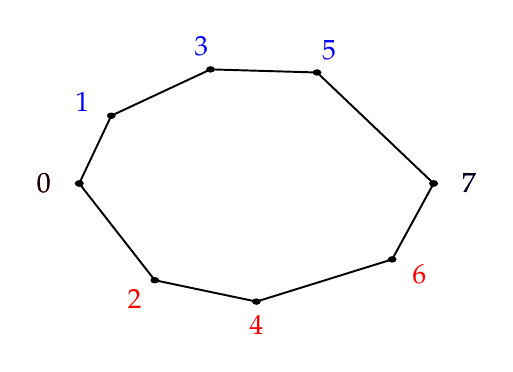
\begin{tikzpicture}[xscale=1.5]
            \foreach \x/\i in {180/0,235/2,270/4,320/6} {
            \draw[line width=.7pt,black,fill=black] (\x:1.5cm) coordinate (x\i) circle (.8pt);
            \node at (\x:1.8cm) {\color{red} \i};}
            
            \foreach \x/\i in {145/1,105/3,70/5,360/7} {
            \draw[line width=.7pt,black,fill=black] (\x:1.5cm) coordinate (x\i) circle (.8pt);
            \node at (\x:1.8cm) {\color{blue} \i};}

            \foreach \x/\i in {360/7} {
            \draw[line width=.7pt,black,fill=black] (\x:1.5cm) coordinate (x\i) circle (.8pt);
            \node at (\x:1.8cm) {\color{black} \i};}
            
            \foreach \x/\i in {180/0} {
            \draw[line width=.7pt,black,fill=black] (\x:1.5cm) coordinate (x\i) circle (.8pt);
            \node at (\x:1.8cm) {\color{black} \i};}

            \draw [line width=.7pt,black] (x0) -- (x2) -- (x4) -- (x6) -- (x7) -- (x5) -- (x3) -- (x1) -- cycle;
        \end{tikzpicture}
    \end{figure}
    
    \begin{itemize}
        \item Draw a polygon with $n+2$ vertices
        \item Label vertices \textcolor{blue}{odd} and \textcolor{red}{even} as above
    \end{itemize}
\end{frame}

\begin{frame}{The Elements: Triangulations}
    \begin{figure}
        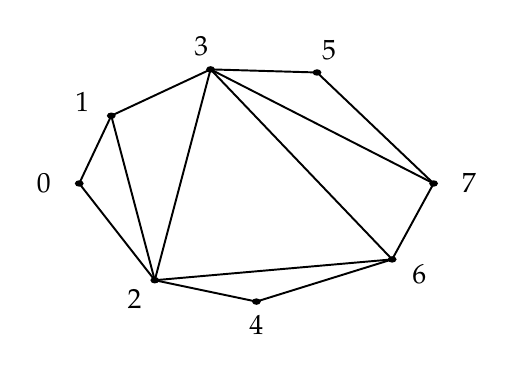
\begin{tikzpicture}[xscale=1.5]
            \foreach \x/\i in {180/0,235/2,270/4,320/6,145/1,105/3,70/5,360/7} {
            \draw[line width=.7pt,black,fill=black] (\x:1.5cm) coordinate (x\i) circle (.8pt);
            \node at (\x:1.8cm) {\i};}

            \draw [line width=.7pt,black] (x0) -- (x2) -- (x4) -- (x6) -- (x7) -- (x5) -- (x3) -- (x1) -- cycle;

            \draw [line width=.7pt,black] (x1) -- (x2);
            \draw [line width=.7pt,black] (x2) -- (x3);
            \draw [line width=.7pt,black] (x2) -- (x6);
            \draw [line width=.7pt,black] (x3) -- (x6);
            \draw [line width=.7pt,black] (x3) -- (x7);

            % draw some lines inside this
        \end{tikzpicture}
    \end{figure}
    
    \begin{itemize}
        \item Triangulate the polygon \\ \pause
        \item \textbf{\emph{These triangulations are the elements in our poset!}}
    \end{itemize}
\end{frame}

% \begin{frame}{Defining: Comparable elements}
%     \begin{figure}
%     \centering
%         \begin{subfigure}{.5\textwidth}
%         \centering
%         \includegraphics[width=0.6\linewidth]{Capture_LI (4).jpg}
%         \end{subfigure}%
%         \begin{subfigure}{.5\textwidth}
%         \centering
%         \includegraphics[width=0.6\linewidth]{Capture2_LI (2).jpg}
%         \end{subfigure}
%     \caption{Two comparable triangulations}
%     \label{fig:test}
%     \end{figure}
    
%     \begin{itemize}
%         \item Triangulations are comparable if they differ by a sequence of (something) diagonal flips
%     \end{itemize}
% \end{frame}

\begin{frame}{Defining: Comparable Elements}
    \begin{columns}

    \begin{column}{0.4\textwidth}
        \phantom{foo}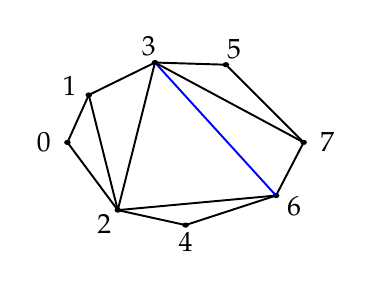
\begin{tikzpicture}[xscale=1.0, yscale=.7]
            \foreach \x/\i in {180/0,235/2,270/4,320/6,145/1,105/3,70/5,360/7} {
            \draw[line width=.7pt,black,fill=black] (\x:1.5cm) coordinate (x\i) circle (.8pt);
            \node at (\x:1.8cm) {\i};}

            \draw [line width=.7pt,black] (x0) -- (x2) -- (x4) -- (x6) -- (x7) -- (x5) -- (x3) -- (x1) -- cycle;

            \draw [line width=.7pt,black] (x1) -- (x2);
            \draw [line width=.7pt,black] (x2) -- (x3);
            \draw [line width=.7pt,black] (x2) -- (x6);
            \draw [line width=.7pt,blue] (x3) -- (x6);
            \draw [line width=.7pt,black] (x3) -- (x7);

            % draw some lines inside this
        \end{tikzpicture}
    \end{column}
    
    \begin{column}{0.2\textwidth}
    
    \vspace{-2.4 cm}
    
    %\begin{center}
        \phantom{a} \Huge \boldmath $\leq$
    %\end{center}
        
    \end{column}
    \begin{column}{0.4\textwidth}  %%<--- here
        \hspace{-1 cm} 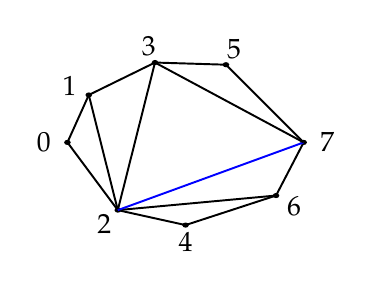
\begin{tikzpicture}[xscale=1.0, yscale = .7]
            \foreach \x/\i in {180/0,235/2,270/4,320/6,145/1,105/3,70/5,360/7} {
            \draw[line width=.7pt,black,fill=black] (\x:1.5cm) coordinate (x\i) circle (.8pt);
            \node at (\x:1.8cm) {\i};}

            \draw [line width=.7pt,black] (x0) -- (x2) -- (x4) -- (x6) -- (x7) -- (x5) -- (x3) -- (x1) -- cycle;

            \draw [line width=.7pt,black] (x1) -- (x2);
            \draw [line width=.7pt,black] (x2) -- (x3);
            \draw [line width=.7pt,black] (x2) -- (x6);
            \draw [line width=.7pt,blue] (x2) -- (x7);
            \draw [line width=.7pt,black] (x3) -- (x7);

            % draw some lines inside this
        \end{tikzpicture}
    \end{column}
    \end{columns}
    \vspace{0.8cm}
    \begin{itemize}
        \item Two polygons sharing an arrow differ by one \textbf{diagonal flip}
        \item Arrow points towards polygon with the more positive diagonal
    \end{itemize}
\end{frame}

\begin{frame}{Bipartite Cambrian Lattice}
        \begin{figure}
        \centering
            \includegraphics[scale = .6]{ExCambrianLattice.png}
        \caption*{\textcolor{blue}{\textbf{[Reading; 2012]}}}
        \end{figure}
    
    \emph{\textbf{Note: Elements listed higher in the poset have higher-sloped diagonals}}
    
    % \begin{itemize}
    %     \item Bipartite polygons ordered by diagonal flips
    %     \item Polygons with higher slope are placed towards the top of the diagram
    % \end{itemize}
\end{frame}

\begin{frame}{Chains and antichains}
   \vspace{-1cm}
    \begin{columns}
    
        \begin{column}{0.5\textwidth}
            \begin{figure}
                \centering
                \includegraphics[scale = 0.3]{ExA.png}
            \end{figure}
            \begin{itemize}
                \item \textbf{Chain}: A subset in which every pair of elements is comparable
                
                \item \textbf{Chain Size}: \# elements in the chain
            \end{itemize}
        \end{column}
        
        
        
        \begin{column}{0.5\textwidth}
            \begin{figure}
                \centering
                \includegraphics[scale = 0.08]{Antichain_B.PNG}
            \end{figure}
            
            \begin{itemize}
                \item \textbf{Antichain}: A subset in which every pair of elements is incomparable
                
                \item \textbf{Antichain Size}: \# elements in the antichain
            \end{itemize}
        \end{column}
        
    \end{columns}
\end{frame}

% \begin{frame}{Poset: Chains}
% \vspace{-0.2cm}
%     \begin{figure}
%         \centering
%         \includegraphics[width=6cm]{ExA.png}
%     \end{figure}
%     \begin{itemize}
%          \item \textbf{Chain}: Totally ordered subset of a poset
%          \item \textbf{Chain Size}: Number of elements in the chain
%      \end{itemize}
% \end{frame}
    
% \begin{frame}{Poset: antichains}
%      \begin{figure}
%          \centering
%          \includegraphics[width=5cm]{antichains.png}
%      \end{figure}
%      \begin{itemize}
%          \item \textbf{antichain}: A subset of a poset in which any two distinct elements are incomparable
%          \item \textbf{antichain Size}: Number of elements in the antichain
%      \end{itemize}
% \end{frame}

% \begin{frame}{Greene-Kleitman Theorem}

%      \textbf{Theorem} (\emph{Greene-Kleitman})
%      \begin{itemize}
%          \item $A_k$ = size of the largest union of $k$ chains of $P$
%          \item $D_k$ = size of the largest union of $k$ antichains of $P$
%          \item $\lambda_k$ = $A_{k+1} - A_k$ for all $k$, and $\lambda := (\lambda_1, \lambda_2,...)$
%          \item $\mu_k$ = $D_{k+1} - D_k$ for all $k$, and $\mu := (\mu_1, \mu_2,...)$
%      \end{itemize}
%      Then, $\lambda$ and $\mu$ are partitions, and they are conjugate.
%  \end{frame}
 
%  \begin{frame}{Greene-Kleitman Theorem}
%     \textbf{Theorem} (\emph{Greene-Kleitman})
%      \begin{itemize}
%          \item $A_k$ = size of the largest union of $k$ chains of $P$
%          \item $D_k$ = size of the largest union of $k$ antichains of $P$
%          \item \colorbox{yellow}{$\mu_k$ = $D_{k+1} - D_k$ for all $k$, and $\mu := (\mu_1, \mu_2,...)$}
%          \item $\mu_k$ = $D_{k+1} - D_k$ for all $k$, and $\mu := (\mu_1, \mu_2,...)$
%      \end{itemize}
%      Then, $\lambda$ and $\mu$ are partitions, and they are conjugate.
%  \end{frame}
    

% \begin{frame}{Research Results}
%     \begin{figure}
%         \centering
%         % \includegraphics[width=5cm]{lattice.png}
%         \includegraphics[scale = 0.07]{lattice.png}
%     \end{figure}
%     \textbf{Question:} What is $\lambda$ for the Bipartite Cambrian Poset? \\
%     \vspace{0.5cm}
%     \textbf{Answer:} The first $\lfloor\frac{n-1}{2}\rfloor$ parts are given below as such:
%     \begin{center}
%         $\lambda_1 - 2 = \lambda_2 = \lambda_3 = \cdots = \lambda_{\lfloor\frac{n-1}{2}\rfloor} > \lambda_{\lfloor\frac{n-1}{2}\rfloor + 1}$
%     \end{center}
% \end{frame}


\begin{frame}{Research Problem}
    \begin{center}
        \includegraphics[scale = .3]{ExA.png}
    \end{center}

    \textbf{Question:} For all $n$, how many maximum-length chains share only their first and last elements?\\ \pause
    \vspace{0.5cm}
    \textbf{Theorem:} The maximum attainable number is $\lfloor\frac{n-1}{2}\rfloor$
\end{frame}

\begin{frame}{One key idea: focus on a special subposet}
    \begin{center}
        \includegraphics[scale = .105]{lattice.png}
    \end{center}
\end{frame}

\begin{frame}

    \vspace{1 cm}

    \begin{center}
        \Huge
        \textbf{Part 2}\\
        The Tamari Lattice
    \end{center}
\end{frame}
 
\begin{frame}{Creating the Tamari Lattice}
    \begin{figure}
        \centering
        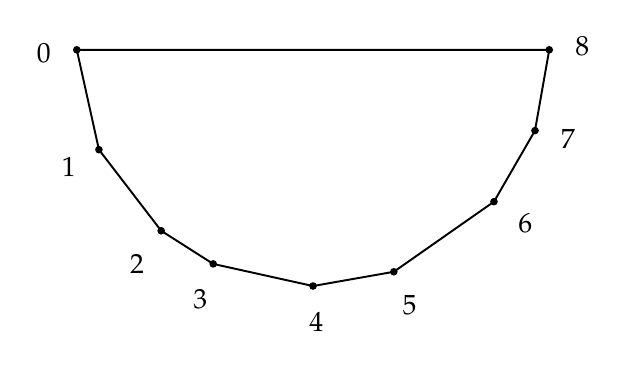
\begin{tikzpicture}[scale=2]
            \foreach \x/\i in {180/0,205/1,230/2,245/3,270/4,290/5,320/6,340/7,360/8} {
            \draw[line width=.7pt,black,fill=black] (\x:1.5cm) coordinate (x\x) circle (.5pt); 
            \node[anchor=180+\x] at ($(x\x)+(\x+11.25:3pt)$) {\i};}
            
            \draw [line width=.7pt,black] (x180) -- (x205) -- (x230) -- (x245) -- (x270) -- (x290) -- (x320) -- (x340) -- (x360) -- cycle;

        \end{tikzpicture}
    \end{figure}
    \begin{itemize}
        \item Draw a polygon with $n+2$ vertices
        \item Label vertices in increasing order
    \end{itemize}
    
    {\color{blue} Note: The only difference from before is how we order the vertices!}
\end{frame}

\begin{frame}{Creating the Tamari Lattice}
    \begin{figure}
        \centering
        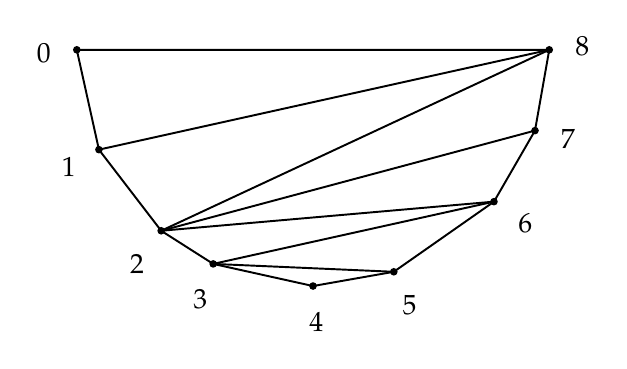
\begin{tikzpicture}[scale=2]
            \foreach \x/\i in {180/0,205/1,230/2,245/3,270/4,290/5,320/6,340/7,360/8} {
            \draw[line width=.7pt,black,fill=black] (\x:1.5cm) coordinate (x\x) circle (.5pt); 
            \node[anchor=180+\x] at ($(x\x)+(\x+11.25:3pt)$) {\i};}
            
            \draw [line width=.7pt,black] (x180) -- (x205) -- (x230) -- (x245) -- (x270) -- (x290) -- (x320) -- (x340) -- (x360) -- cycle;

            \draw [line width=.7pt,black] (x205) -- (x360);
            \draw [line width=.7pt,black] (x230) -- (x360);
            \draw [line width=.7pt,black] (x230) -- (x340);
            \draw [line width=.7pt,black] (x230) -- (x320);
            \draw [line width=.7pt,black] (x245) -- (x320);
            \draw [line width=.7pt,black] (x245) -- (x290);
        \end{tikzpicture}
    \end{figure}
    
    \begin{itemize}
        \item Triangulate the polygon
        \item \textbf{\emph{These triangulations are the elements in our poset!}}
    \end{itemize}
\end{frame}

\begin{frame}{The Tamari Lattice}
    \begin{figure}
        \centering
        \includegraphics[scale = 0.7]{Capture1.PNG}
    \end{figure}
    \emph{\textbf{Note: As before, elements listed higher in the poset have higher-sloped diagonals}}
\end{frame}

\begin{frame}{Research Results}
     \begin{figure}
         \centering
         \includegraphics[scale = 0.08]{antichains_T.PNG}
     \end{figure}
     \textbf{Question:} For all $n$, what is the size of the largest antichain? \pause

        % \item \textbf{Theorem:} The size $T$ satisfies
        % $$\Omega\left(\frac{2^{n/2}}{\sqrt{n}}\right) \le T \le O\left(\frac{2^n}{n^{3/2}}\right)$$

      \textbf{Theorem:} The largest antichain has size at least \\
         
      \Large $$\binom{\lfloor\frac{n}{2}\rfloor}{\lfloor\frac{n}{4}\rfloor} \approx   \frac{2^{n/2}}{\sqrt{n}}$$
\end{frame}

\begin{frame}{Key Idea: Flip only certain ``special'' lines}
    \begin{columns}
    \begin{column}{0.5\textwidth}
    \begin{figure}
        \centering
        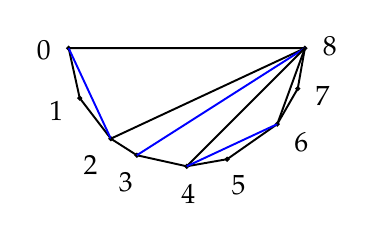
\begin{tikzpicture}[scale=1]
            \foreach \x/\i in {180/0,205/1,230/2,245/3,270/4,290/5,320/6,340/7,360/8} {
            \draw[line width=.7pt,black,fill=black] (\x:1.5cm) coordinate (x\x) circle (.5pt); 
            \node[anchor=180+\x] at ($(x\x)+(\x+11.25:3pt)$) {\i};}
            
            \draw [line width=.7pt,black] (x180) -- (x205) -- (x230) -- (x245) -- (x270) -- (x290) -- (x320) -- (x340) -- (x360) -- cycle;

            \draw [line width=.7pt,blue] (x180) -- (x230);
            \draw [line width=.7pt,black] (x230) -- (x360);
            \draw [line width=.7pt,blue] (x245) -- (x360);
            \draw [line width=.7pt,black] (x270) -- (x360);
            \draw [line width=.7pt,blue] (x270) -- (x320);
            \draw [line width=.7pt,black] (x320) -- (x360);
        \end{tikzpicture}
    \end{figure}
    
    \begin{figure}
        \centering
        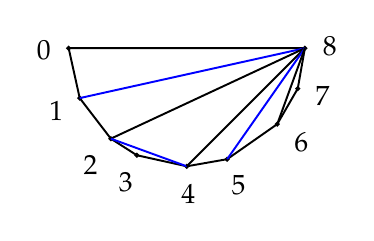
\begin{tikzpicture}[scale=1]
            \foreach \x/\i in {180/0,205/1,230/2,245/3,270/4,290/5,320/6,340/7,360/8} {
            \draw[line width=.7pt,black,fill=black] (\x:1.5cm) coordinate (x\x) circle (.5pt); 
            \node[anchor=180+\x] at ($(x\x)+(\x+11.25:3pt)$) {\i};}
            
            \draw [line width=.7pt,black] (x180) -- (x205) -- (x230) -- (x245) -- (x270) -- (x290) -- (x320) -- (x340) -- (x360) -- cycle;

            \draw [line width=.7pt,blue] (x205) -- (x360);
            \draw [line width=.7pt,black] (x230) -- (x360);
            \draw [line width=.7pt,blue] (x230) -- (x270);
            \draw [line width=.7pt,black] (x270) -- (x360);
            \draw [line width=.7pt,blue] (x290) -- (x360);
            \draw [line width=.7pt,black] (x320) -- (x360);
        \end{tikzpicture}
    \end{figure}
    \end{column}
    
    \begin{column}{0.5\textwidth}
    \begin{figure}
        \centering
        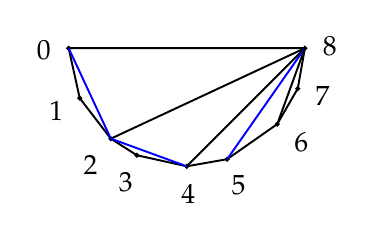
\begin{tikzpicture}[scale=1]
            \foreach \x/\i in {180/0,205/1,230/2,245/3,270/4,290/5,320/6,340/7,360/8} {
            \draw[line width=.7pt,black,fill=black] (\x:1.5cm) coordinate (x\x) circle (.5pt); 
            \node[anchor=180+\x] at ($(x\x)+(\x+11.25:3pt)$) {\i};}
            
            \draw [line width=.7pt,black] (x180) -- (x205) -- (x230) -- (x245) -- (x270) -- (x290) -- (x320) -- (x340) -- (x360) -- cycle;
            
            \draw [line width=.7pt,blue] (x180) -- (x230);
            \draw [line width=.7pt,black] (x230) -- (x360);
            \draw [line width=.7pt,blue] (x230) -- (x270);
            \draw [line width=.7pt,black] (x270) -- (x360);
            \draw [line width=.7pt,blue] (x290) -- (x360);
            \draw [line width=.7pt,black] (x320) -- (x360);
        \end{tikzpicture}
    \end{figure}
    
    \begin{figure}
        \centering
        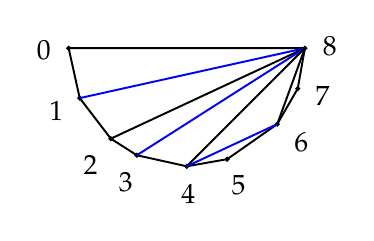
\begin{tikzpicture}[scale=1]
            \foreach \x/\i in {180/0,205/1,230/2,245/3,270/4,290/5,320/6,340/7,360/8} {
            \draw[line width=.7pt,black,fill=black] (\x:1.5cm) coordinate (x\x) circle (.5pt); 
            \node[anchor=180+\x] at ($(x\x)+(\x+11.25:3pt)$) {\i};}
            
            \draw [line width=.7pt,black] (x180) -- (x205) -- (x230) -- (x245) -- (x270) -- (x290) -- (x320) -- (x340) -- (x360) -- cycle;

            \draw [line width=.7pt,blue] (x205) -- (x360);
            \draw [line width=.7pt,black] (x230) -- (x360);
            \draw [line width=.7pt,blue] (x245) -- (x360);
            \draw [line width=.7pt,black] (x270) -- (x360);
            \draw [line width=.7pt,blue] (x270) -- (x320);
            \draw [line width=.7pt,black] (x320) -- (x360);
        \end{tikzpicture}
    \end{figure}
    \end{column}
    \end{columns}
\end{frame}

\begin{frame}{Greene-Kleitman Theorem}
    \vspace{-0.9cm}
    \begin{columns}
        \begin{column}{0.5\textwidth}
            \begin{figure}
                \centering
                \includegraphics[scale = 0.25]{ExA.png}
            \end{figure}
        \end{column}
        \begin{column}{0.5\textwidth}
            \begin{figure}
                \centering
                \includegraphics[scale = 0.07]{Antichain_B.PNG}
            \end{figure}
        \end{column}
    \end{columns}
    
    \vspace{0.5cm}
    
    \textbf{Theorem} \textcolor{blue}{[Greene, Kleitman; 1976]}
     \begin{itemize}
         \item $A_k$ = size of the largest union of $k$ chains of $P$ ($A_0 = 0$) 
         \item $D_k$ = size of the largest union of $k$ antichains of $P$ ($D_0 = 0$)
         \item $\lambda_k$ = $A_{k} - A_{k-1}$ for all $k$, and $\lambda := (\lambda_1, \lambda_2,...)$
         \item $\mu_k$ = $D_{k} - D_{k-1}$ for all $k$, and $\mu := (\mu_1, \mu_2,...)$
     \end{itemize}
     Then, $\lambda$ and $\mu$ are partitions, and they are conjugate.
 \end{frame}

\begin{frame}{Our Theorems Rewritten}
    \vspace{1cm}
    \begin{enumerate}
        \item Largest union of disjoint chains in Bipartite Cambrian Lattice: 
        \begin{center} \Large
            $\lambda_1 - 2 = \lambda_2 = \lambda_3 = \cdots = \lambda_{\lfloor\frac{n-1}{2}\rfloor} > \lambda_{\lfloor\frac{n-1}{2}\rfloor + 1}$
        \end{center}
    
    \vspace{0.5cm}
    
        \item Largest antichain in Tamari Lattice:
        \vspace{0.3cm}
        \begin{center}
           \Large $\mu_1 \ge \frac{2^{n/2}}{\sqrt{n}}$
        \end{center}
    \end{enumerate}
\end{frame}

\begin{frame}

    \vspace{1 cm}

    \begin{center}
        \Huge
        \textbf{Thank You!}\\
    \end{center}
\end{frame}

% \begin{frame}{References}
%     \bibliographystyle{alpha}
%     \bibliography{bib}{}    
% \end{frame}

\end{document}
